\section{Present records and later responses}\label{sec:records}
A census, an offset, a threshold ladder and a gas state are present records. This section asks which later quantities a present record fixes, and answers with exact witnesses: in each, two preparations agree on a declared record and disagree on a declared later readout, and the lost distinction is named. A complete state evolves deterministically; what fails is the sufficiency of the summary.

\subsection{Retained and hidden amplitudes}
Let $\mathcal H=\mathcal H_A\oplus\mathcal H_B$ be finite-dimensional, $H=\begin{pmatrix}A&B\\B^\dagger&D\end{pmatrix}=H^\dagger$, $\psi=(x,y)$, $i\hbar\dot\psi=H\psi$. The partition is physical data; if it is an invariant spectral subspace of $H$ then $B=0$.

\begin{theorem}[the reduced equation, with the hidden source]\label{thm:reduced}
With $K(t)=Be^{-iDt/\hbar}B^\dagger$ and $J(t)=Be^{-iDt/\hbar}y(0)$,
\[
\dot x(t)=-\frac i\hbar Ax(t)-\frac i\hbar J(t)-\frac1{\hbar^2}\int_0^tK(t-s)x(s)\,ds.
\]
$A$, $K$, $J$ and $x(0)$ determine the retained evolution; a kernel without the source term does not when $y(0)\neq0$. If $E_D$ is the spectral measure of $D$, $d\mathsf M(\lambda)=B\,dE_D(\lambda)\,B^\dagger$ is a positive operator-valued measure with $K(t)=\int e^{-i\lambda t/\hbar}d\mathsf M$, $\Sigma(z)=B(z-D)^{-1}B^\dagger=\int d\mathsf M/(z-\lambda)$, and the retained resolvent is $G_A(z)=(z-A-\Sigma(z))^{-1}$. $K(0)=\mathsf M(\mathbb R)=BB^\dagger$ is the total channel mass, not its frequency distribution; $\Ima\Sigma(z)\le0$ for $\Ima z>0$; and $\sum_{j,k}u_j^\dagger K(t_j-t_k)u_k=\|\sum_ke^{iDt_k/\hbar}B^\dagger u_k\|^2\ge0$. \grade{T}
\end{theorem}
\begin{proof}
Variation of constants in the hidden equation, $y(t)=e^{-iDt/\hbar}y(0)-\frac i\hbar\int_0^te^{-iD(t-s)/\hbar}B^\dagger x(s)ds$, substituted in $\dot x=-\frac i\hbar(Ax+By)$. The spectral theorem gives the integrals and the positivity of each atom $BE_D(\{\lambda\})B^\dagger$; block elimination gives the Schur inverse; $\Ima\Sigma=-(\Ima z)B((\Rea z-D)^2+(\Ima z)^2)^{-1}B^\dagger$.
\end{proof}
The footprint $K(0)=BB^\dagger$ is the weight between of §\ref{sec:cross} for the generator. These properties constrain admissible kernels; they do not turn a scalar delay curve into a reconstructed measure.

\begin{proposition}[equal spectrum, equal footprint, different survival]\label{prop:R3}
Set $\hbar=1$, $\Lambda=\mathrm{diag}(-3,-1,1,3)$, $w^{(0)}=(1,1,1,1)/4$, $w^{(1)}=(3,7,1,5)/16$. For each, $s=(\sqrt{w_j})$, $v=e_0-s$, $R_w=I-vv^T/(1-s_0)$ (a reflection with $R_we_0=s$), $H_w=R_w\Lambda R_w^T$. Both Hamiltonians have spectrum $\{-3,-1,1,3\}$, retained block $A=0$ and footprint $BB^T=5$; from $\psi(0)=e_0$ their retained survivals at $t=\pi/4$ are $0$ and $1/32$. \grade{T}\grade{V}
\end{proposition}
\begin{proof}
$v^Tv=2(1-s_0)$ makes $R_w$ an orthogonal reflection. The amplitude is $a_w(t)=\sum_jw_je^{-i\lambda_jt}$. Both weight vectors have $\sum w\lambda=0$ and $\sum w\lambda^2=5$, which give $A=0$ and $BB^T=5$. For $w^{(0)}$, $a_0=(\cos3t+\cos t)/2$; the difference weights $(-1,3,-3,1)/16$ give $a_1-a_0=\frac i8(3\sin t-\sin3t)=\frac i2\sin^3t$. At $t=\pi/4$, $a_0=0$, $a_1=i\sqrt2/8$.
\end{proof}
The third moments are $0$ and $3$: $BDB^T$ is $0$ and $3$, so $K'(0)=-iBDB^T$ differs while $K(0)$ agrees. The retained resolvents are $G_0=(z^3-5z)/Q$ and $G_1=(z^3-5z+3)/Q$ with $Q=(z^2-1)(z^2-9)$, and $\Sigma_0=(5z^2-9)/(z^3-5z)$, $\Sigma_1=(5z^2+3z-9)/(z^3-5z+3)$: both begin $5/z$ at large $z$ and part at the next coefficient.

\begin{proposition}[same kernel, different hidden source]\label{prop:R4}
$H=\sigma_x$, $\psi_\pm(0)=(1,\pm i)/\sqrt2$: equal retained amplitude at $t=0$, $A=D=0$, $K(t)=1$, yet $|x_\pm(t)|^2=\tfrac12(1\pm\sin2t)$, so $1$ and $0$ at $t=\pi/4$; the hidden sources are $J_\pm=\pm i/\sqrt2$. \grade{T}
\end{proposition}
\begin{proof}
$e^{-iHt}=\cos t\,I-i\sin t\,H$ gives $x_\pm=(\cos t\pm\sin t)/\sqrt2$.
\end{proof}
Proposition~\ref{prop:R4} changes the initial state; Proposition~\ref{prop:R3} keeps it and changes the spectral weights. They are two separate omissions, and Proposition~\ref{prop:joint} is the first of them seen through the offset.

\subsection{A finite moment record}
\begin{theorem}[matched moments, different response]\label{thm:moments}
Let $m\ge1$, $x_j=a+jh$ ($h\neq0$, $0\le j\le m$), $p_j>0$ with $\sum p_j=1$, $w_j=(-1)^j\binom mj$, $q_j=p_j+\delta w_j$ with $0<|\delta|<\min_jp_j/|w_j|$. Then $p\neq q$ are positive probability vectors with equal moments of every order $r<m$, $\sum_j(q_j-p_j)x_j^m=\delta(-1)^mm!h^m$, and $F_q(t)-F_p(t)=\delta e^{-iat}(1-e^{-iht})^m$ for $F_p(t)=\sum p_je^{-itx_j}$. No rule of the first $m$ moments reproduces the whole response. \grade{T}\grade{L}($m=3$ witness)
\end{theorem}
\begin{proof}
$\sum w_j=(1-1)^m=0$. The $m$-th forward difference annihilates polynomials of degree below $m$ and returns $m!h^m$ on $x^m$. The exponential sum is a binomial expansion; its real zeros are the recurrence times $ht\in2\pi\mathbb Z$.
\end{proof}
The readout matters as well. For $m=3$ on $(-3,-1,1,3)$, the uniform weights and $(3,7,1,5)/16$ share normalisation, mean $0$ and second moment $5$, and their intensities at $t=\pi/4$ are $0$ and $1/32$; the reflected weights $(5,1,7,3)/16$ have the complex-conjugate response and the same intensity at every real time (Figure~\ref{fig:futures}, left). An intensity-only detector erases what a phase-resolved one keeps. The anchored VOTKP ladder is a different case: it is an invertible coordinate of the complete threshold list (Theorem~\ref{thm:anchor}), and nothing is lost in that map; the missing response data are the preparation and channel weights the list never claimed to hold. Exact rational checks at orders $1$ through $12$ hold with residuals at most $3.3\times10^{-16}$ \grade{V}.

\subsection{A gas witness: same density, flow and stress}
\begin{theorem}[kinetic witness]\label{thm:kinetic}
On a period $L$ with $k=2\pi m/L$, fix $\rho_*>0$, $0<\eta<1$, $v_0>0$, $0<a<1/12$, $\sigma\ge0$; $u=(-3,-1,1,3)$, $d=(-1,3,-3,1)$, $\rho(x)=\rho_*[1+\eta\cos kx]$, $g_\sigma$ the centred Gaussian of variance $\sigma^2$ (a point mass at $\sigma=0$), $p_\pm(v)=\sum_j(\tfrac14\pm ad_j)g_\sigma(v-v_0u_j)$ and $f_\pm(x,v,0)=\rho(x)p_\pm(v)$.
\begin{enumerate}
\item (K1) Pointwise $M_0^\pm=\rho$, $M_1^\pm=0$, $M_2^\pm=(5v_0^2+\sigma^2)\rho$, but $M_3^\pm=\pm48av_0^3\rho$.
\item (K2) Under the same free streaming $\partial_tf+v\partial_xf=0$, with $q=kv_0t$,
\begin{gather*}
n_\pm=\rho_*\big[1+\eta e^{-\sigma^2k^2t^2/2}\big(\tfrac12[\cos q+\cos3q]\cos kx\mp8a\sin^3q\sin kx\big)\big],\\
\Delta n=-16a\eta\rho_*e^{-\sigma^2k^2t^2/2}\sin kx\sin^3(kv_0t).
\end{gather*}
\item (K3) $\Delta n=\partial_t\Delta n=\partial_t^2\Delta n=0$ at $t=0$, while $\partial_t^3\Delta n=-\partial_x^3\Delta M_3=-96a\eta\rho_*k^3v_0^3\sin kx$.
\item (K4) The pre-release reset $\mathcal E_s[f]=e^{-\nu s}f+(1-e^{-\nu s})\rho p_0$, $p_0=\frac14\sum_jg_\sigma(v-v_0u_j)$, preserves density, flow, stress and positivity and multiplies the later contrast by exactly $e^{-\nu s}$. \grade{T}
\end{enumerate}
\end{theorem}
\begin{proof}
$\sum d_j=0$ and $\min(\tfrac14\pm ad_j)=\tfrac14-3a>0$. Exact sums: $\sum d_ju_j^\ell=0$ for $\ell\le2$ and $48$ for $\ell=3$; convolution adds $\sigma^2$ to second moments and $3\sigma^2v_0u_j$ to third, whose $d$-weighted sum vanishes. Characteristics give $f(x-vt,v,0)$; the Gaussian transform gives $e^{-ikv_0u_jt}e^{-\sigma^2k^2t^2/2}$; $\sum d_j\cos qu_j=0$ and $\sum d_j\sin qu_j=2\sin3q-6\sin q=-8\sin^3q$. The moment hierarchy $\partial_tM_\ell+\partial_xM_{\ell+1}=0$ iterated three times gives K3. The reset is a convex combination of positive distributions with equal first three moments and is linear.
\end{proof}
At $a=1/24$, $\eta=\tfrac12$, $\rho_*=v_0=k=1$, $\sigma=0$, $x=t=\pi/2$: $n_+=5/6$, $n_-=7/6$, $\Delta n=-1/3$ (Figure~\ref{fig:futures}, right). Stress separates first through its derivative, flow next, density at third order. The full kinetic state is Markovian; history dependence appears only after the higher velocity structure is discarded. The reset is a prescribed preparation map, not the self-consistent collision operator of an isolated gas.

\begin{center}\small
\begin{tabular}{p{0.24\textwidth}p{0.3\textwidth}p{0.36\textwidth}}\toprule
control & exact prediction & what it shows\\\midrule
$a=0$ & $f_+=f_-$, $\Delta n=0$ & the hidden distinction removed\\
$\eta=0$ & $\Delta n=0$ always & a homogeneous density cannot read the velocity record\\
$\sin kx=0$ & no contrast there & placement matters\\
$kv_0t\in\pi\mathbb Z$ & no contrast then & a null readout is not equality of states\\
$s\to\infty$, $\nu>0$ & $\Delta n\to0$ & the reset erases what was prepared\\
$M_3$ also recorded & differ at $t=0$ & the three-moment match is no longer the experiment\\
$\sigma>0$ & Gaussian envelope & spread dephases this readout, states still differ\\\bottomrule
\end{tabular}
\end{center}

\begin{figure}[!htbp]\centering
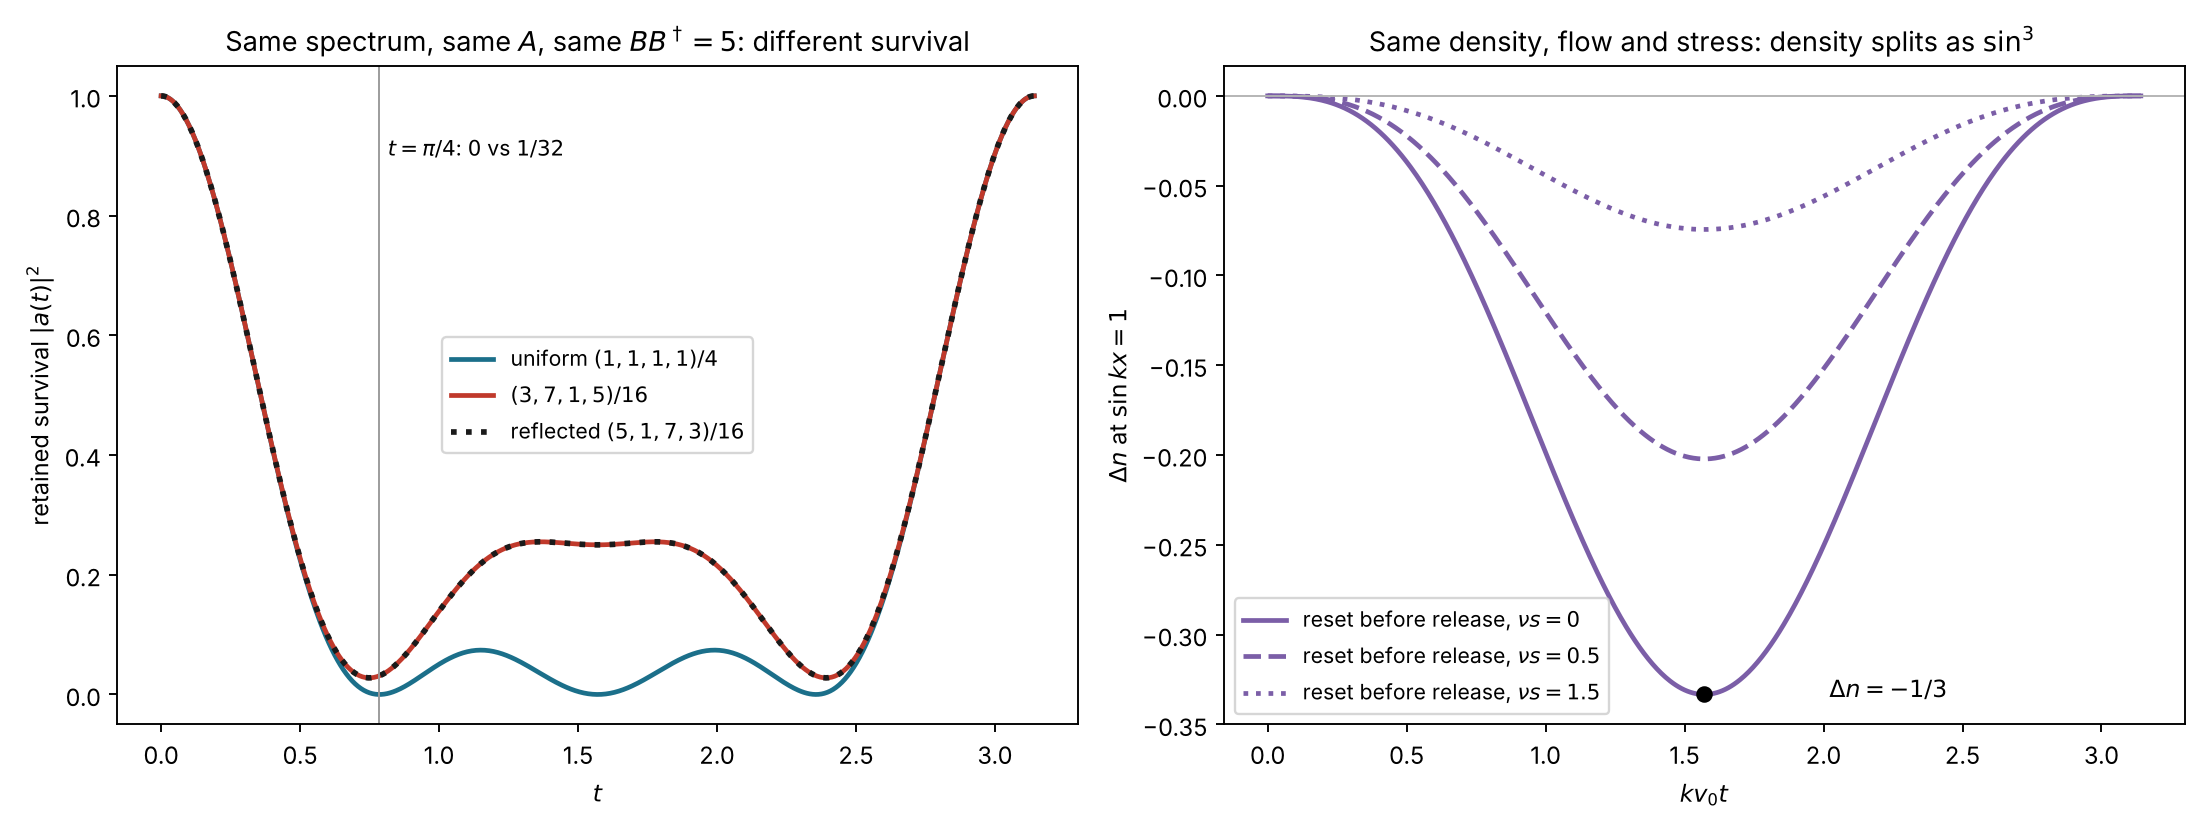
\includegraphics[width=\textwidth]{../figures/fig06_records_and_futures.png}
\caption{Equal present records, different futures. Left: same spectrum, same retained block, same footprint $BB^\dagger=5$, and survival $0$ against $1/32$ at $t=\pi/4$; the reflected weights (dotted) have the same intensity as $(3,7,1,5)/16$ at every time. Right: equal density, flow and stress; free streaming splits density as $-\frac13\sin^3(kv_0t)$ at the exact instance, and a reset before release scales the split by $e^{-\nu s}$.}
\label{fig:futures}
\end{figure}

\subsection{The angular gas chain}
Free streaming in three dimensions, written in normalised Legendre moments of the direction cosine, is the tridiagonal chain $M_{l,l+1}=M_{l+1,l}=c_l=(l+1)/\sqrt{(2l+1)(2l+3)}$. With density-preserving relaxation at rate $\kappa$,
\[
L=-ikM-\kappa(I-P_0),\qquad P_0=e_0e_0^T,
\]
and the density response is $G(s)=\langle e_0,(s-L)^{-1}e_0\rangle$. Four exact results follow, each a card of the angular gas.

\begin{proposition}[ANG1, the free-streaming load]\label{prop:ang1}
At $\kappa=0$, $g_0(s)=\tfrac12\int_{-1}^1\frac{d\mu}{s+ik\mu}=\frac{\arctan(k/s)}{k}$, and the load the hidden moments present to density, $Z_b(s)=1/g_0(s)-s$, tends to $2k/\pi$ as $s\to0^+$. \grade{T}
\end{proposition}
\begin{proof}
$\tfrac12\int_{-1}^1\frac{s\,d\mu}{s^2+k^2\mu^2}=\frac1k\arctan\frac ks$; the odd part integrates to zero. As $s\to0^+$, $\arctan(k/s)\to\pi/2$. By Theorem~\ref{thm:reduced}, $g_0=(s-L_{00}-\Sigma)^{-1}$ with $L_{00}=0$, so $Z_b=-\Sigma(s)$ is the Schur load of the moments above density.
\end{proof}
$Z_b(10^{-2},10^{-4},10^{-6})=0.63070,\ 0.636560,\ 0.6366192$ against $2/\pi=0.6366198$ \grade{V}. This is the declared density response and its reference load, not an electromagnetic reflectance.

\begin{proposition}[ANG2, the relaxation pole]\label{prop:ang2}
For $\kappa>0$, $G=g/(1-\kappa g)$ with $g(s)=g_0(s+\kappa)$. An isolated real pole to the right of the continuum, $s^*>-\kappa$, exists iff $\kappa>2k/\pi$, and then $s^*=k\cot(k/\kappa)-\kappa$; at $\kappa=2k/\pi$ it meets the branch point $s=-\kappa$. \grade{T}
\end{proposition}
\begin{proof}
$s-L=(s+\kappa+ikM)-\kappa P_0$, a rank-one change; Sherman–Morrison on $e_0$ gives $G=g/(1-\kappa g)$ with $g=\langle e_0,(s+\kappa+ikM)^{-1}e_0\rangle=g_0(s+\kappa)$. A real pole with $w=s+\kappa>0$ needs $\arctan(k/w)=k/\kappa$, solvable iff $k/\kappa<\pi/2$, giving $w=k\cot(k/\kappa)$; as $\kappa\downarrow2k/\pi$, $w\downarrow0$.
\end{proof}
ANG1 supplies ANG2's threshold: the pole is born where $\kappa$ equals the free-streaming load $2k/\pi$ \grade{T}. Residuals of the pole condition at $\kappa=0.64,0.7,0.916,1,2$ are below $2\times10^{-16}$ \grade{V}. It is not the two-moment exceptional point of a truncated chain.

\begin{proposition}[ANG3, first return]\label{prop:ang3}
A difference planted in moment $l>2$ first reaches the stress moment at order $l-2$ in $t$, with Taylor coefficient $k^{l-2}\prod_{j=2}^{l-1}c_j/(l-2)!$, and first reaches density at order $l$, for every $\kappa\ge0$. \grade{T}
\end{proposition}
\begin{proof}
$(L^q)_{2,l}$ is a sum over walks of length $q$ from $l$ to $2$ on the path graph with loops; every off-diagonal step changes the index by one, so $q\ge l-2$, and the unique shortest walk uses only off-diagonal steps, contributing $(-ik)^{l-2}\prod_{j=2}^{l-1}c_j$. Diagonal $-\kappa$ terms lengthen walks and enter only at higher order. The same argument gives order $l$ for density.
\end{proof}
For $l=3,4,5,8$ the coefficients are $0.507092553$, $0.127775313$, $0.0214031702$, $2.2474\times10^{-5}$, and every lower power vanishes to $10^{-15}$ \grade{V} (Figure~\ref{fig:angular}). This is the predictive quotient realised on a source model: a planted record is invisible to stress for $l-3$ orders and to density for $l-1$.

\begin{proposition}[ANG4, the two books of the chain]\label{prop:ang4}
For every truncation $N\ge2$, $E^-=\tfrac18\|[L,L^\dagger]\|_F^2=k^2\kappa^2/3$, while $E^+=\tfrac18\|L^2-L^{\dagger2}\|_F^2$ grows with $N$. \grade{T}
\end{proposition}
\begin{proof}
With $L=\mathcal A+\mathcal B$, $\mathcal A=-ikM$ anti-Hermitian and $\mathcal B=-\kappa(I-P_0)$ Hermitian, $L^\dagger=-\mathcal A+\mathcal B$ and $[L,L^\dagger]=2[\mathcal A,\mathcal B]=2ik\kappa[M,I-P_0]=-2ik\kappa[M,P_0]$. Only $c_0=1/\sqrt3$ touches $e_0$, so $[M,P_0]=c_0(e_1e_0^T-e_0e_1^T)$ with $\|\cdot\|_F^2=2c_0^2=\tfrac23$. Then $E^-=\tfrac18\cdot4k^2\kappa^2\cdot\tfrac23$.
\end{proof}
At $k=\kappa=1$ \grade{V}:
\begin{center}\small
\begin{tabular}{rcccccc}\toprule
$N$ & 2 & 5 & 20 & 100 & 200 & 400\\\midrule
$E^-$ & $1/3$ & $1/3$ & $1/3$ & $1/3$ & $1/3$ & $1/3$\\
$E^+$ & $0.333$ & $3.444$ & $18.49$ & $98.50$ & $198.50$ & $398.50$\\
$\|L\|_F^2-\sum|\lambda|^2$ & $1.0000$ & $1.0811$ & $1.1556$ & $1.1715$ & $1.173488$ & $1.174462$\\\bottomrule
\end{tabular}
\end{center} The exact $E^-$, the growth of $E^+$ and the numerical convergence trend of the departure are three different statuses; an infinite-dimensional limit of the departure is not claimed.

\begin{figure}[!htbp]\centering
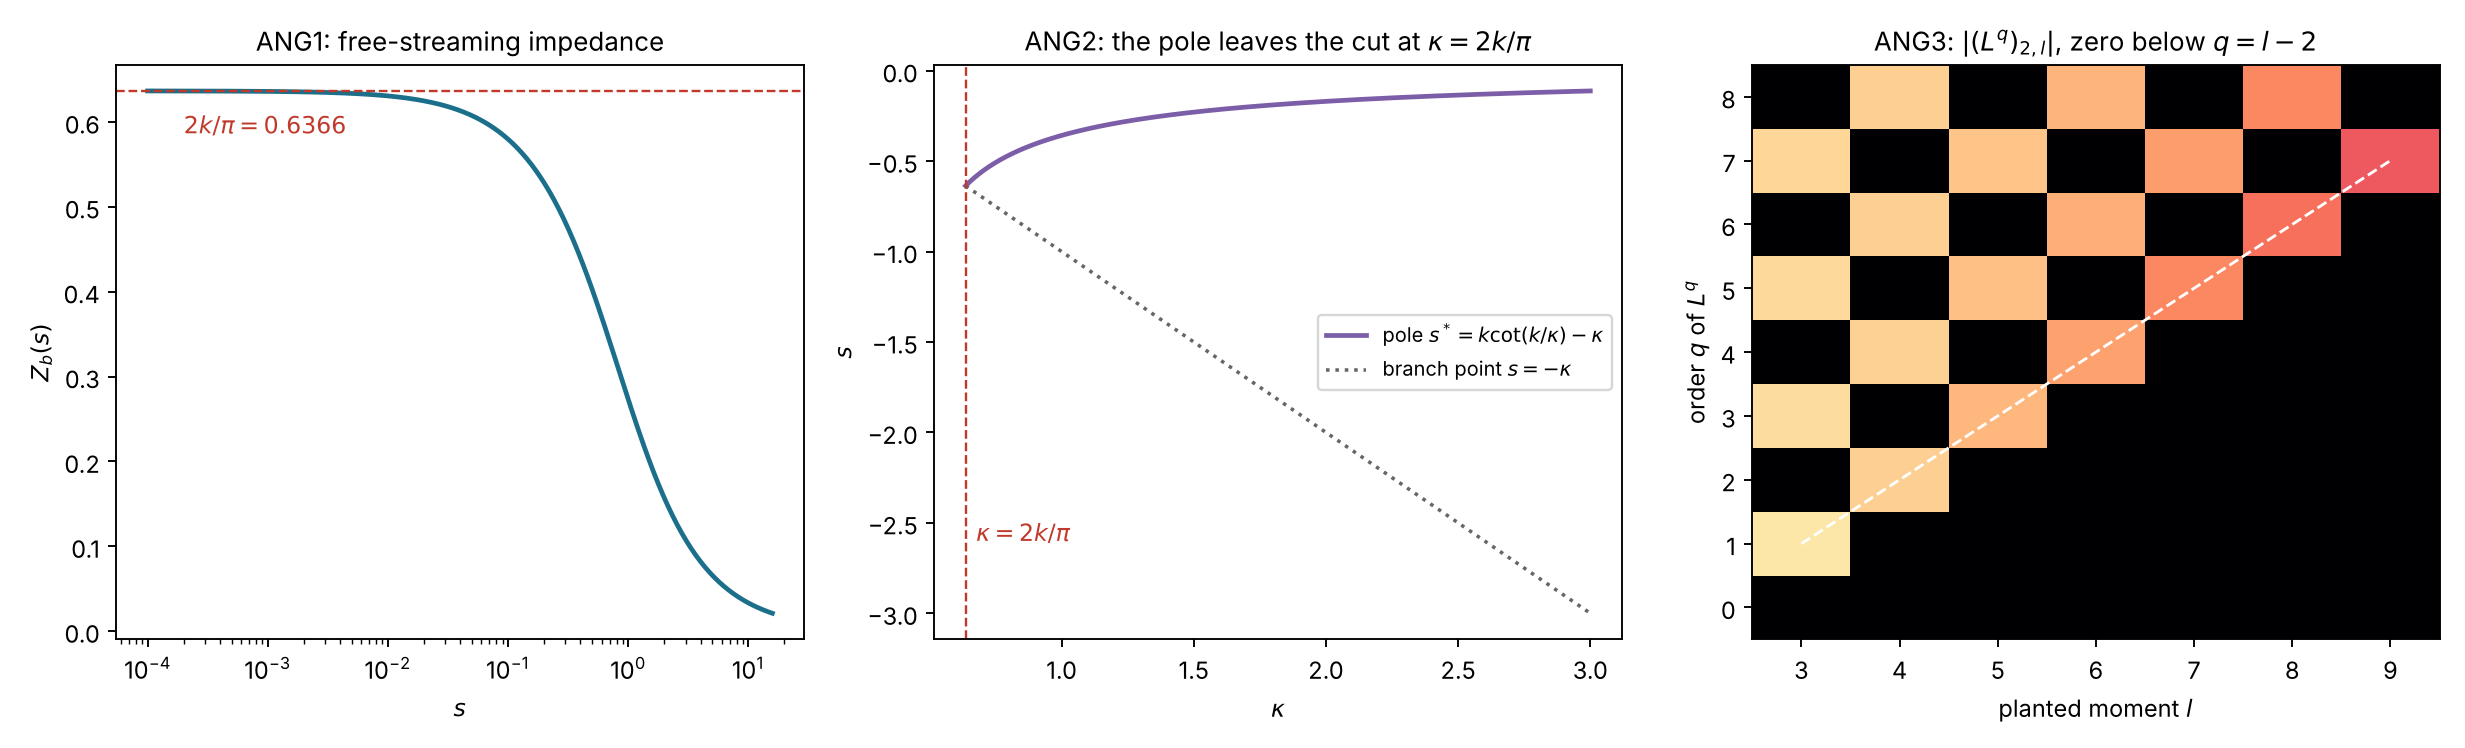
\includegraphics[width=\textwidth]{../figures/fig08_angular_chain.png}
\caption{The angular gas chain ($k=1$). Left: the free-streaming load $Z_b(s)$ tends to $2k/\pi$. Middle: the relaxation pole $s^*=k\cot(k/\kappa)-\kappa$ leaves the branch point at $\kappa=2k/\pi$. Right: $|(L^q)_{2,l}|$ on a log scale; the planted moment reaches stress no sooner than order $l-2$ (dashed).}
\label{fig:angular}
\end{figure}

\section{Opened matter}\label{sec:opened}
\subsection{The opened chain}
Opening matter here means a non-Hermitian effective generator. Take the PT-symmetric SSH chain
\begin{gather*}
h(k)=\begin{pmatrix} iu & v+we^{-ik}\\ v+we^{ik} & -iu\end{pmatrix}=d\cdot\sigma,\\
d=(v+w\cos k,\,w\sin k,\,iu),\qquad s=E(k)^2=d\cdot d=|v+we^{ik}|^2-u^2,
\end{gather*}
with the bilinear dot product. Fill the lower band with the biorthogonal projector $C=\sum_{\mathrm{filled}}|R_k\rangle\langle L_k|$, $\langle L_j|R_k\rangle=\delta_{jk}$, and restrict to a block. The occupations are complex, and so is $\Gamma=1-2\nu$.

\begin{theorem}[what survives opening]\label{thm:open}
Let $C=\begin{pmatrix}A&B\\E&D\end{pmatrix}$ be any idempotent on a finite complex space with a fixed block split, and $Y_A=BE=C_{AB}C_{BA}$. Then $Y_A=A-A^2$, and its eigenvalues are $\nu_j(1-\nu_j)$ with algebraic multiplicity, Jordan blocks allowed. With $R_b(\lambda)=\sqrt{|1-4\lambda|}$, $R_b(\nu(1-\nu))=|1-2\nu|$, so the radial census $\#\{j:R_b(\lambda_j)\le r\}=\#\{j:|1-2\nu_j|\le r\}$ survives for every $r$, and the condition is the disk $|\lambda-\tfrac14|\le r^2/4$. Positivity does not survive: $C=\begin{pmatrix}2&1\\-2&-1\end{pmatrix}$ is idempotent with $Y_A=-2$ and $R_b=3$, and every square $A$ is the compression of the idempotent $\mathcal P(A)=\begin{pmatrix}A&I\\A-A^2&I-A\end{pmatrix}$. \grade{T}\grade{L}
\end{theorem}
\begin{proof}
The $AA$ block of $C^2=C$ is $A^2+BE=A$. Triangularise $A$; the polynomial $z-z^2$ of a triangular matrix has the polynomial of its diagonal on the diagonal. $1-4\nu(1-\nu)=(1-2\nu)^2$. For $\mathcal P(A)$ multiply blocks; every entry is a polynomial in $A$.
\end{proof}
The biorthogonal $C$ of the chain is idempotent to $3\times10^{-14}$, and $|C^2-C|\le2.8\times10^{-14}$, $|X_A-C_A(1-C_A)|\le1.3\times10^{-14}$ in script \texttt{s07} \grade{V}. A principal square root of $(1-2\nu)^2$ returns $\pm(1-2\nu)$, not the modulus; the radial coordinate uses the modulus. The variance and Gaussian readings of §\ref{sec:ledger} need a positive metric and do not come from idempotence; a positive reformulation would need its own inner product, adjoint and partition.

\paragraph{The opened band metric, exactly.} The cone paper (v8) shows that at a Hermitian point the round-trip form $Q=M_{+-}M_{-+}/(E_+-E_-)^2$, $M_{ab}=\langle L_a|\partial h|R_b\rangle$, has $Q\ge0$ (A.13), and measures a Lorentzian cone when the system is opened. The hypothesis is a Hermitian family, or at least a Hermitian tangent: $h(\theta)=\sigma_z+i\theta\sigma_x$ is Hermitian at $\theta=0$ yet has $Q=-\tfrac14$ there. On the opened plane the sign is now exact.

\begin{theorem}[signature of the opened plane]\label{thm:signature}
At fixed real $u,w$, in coordinates $(k,v)$ with $s\neq0$, the bilinear two-level metric $Q_{ab}=[s(\partial_ad\cdot\partial_bd)-(d\cdot\partial_ad)(d\cdot\partial_bd)]/(4s^2)$ is real and
\[
\det Q=-\frac{u^2w^2\cos^2k}{16\,s^3}.
\]
If $s>0$ and $uw\cos k\neq0$ the metric is Lorentzian; if $s<0$ and $uw\cos k\neq0$ it is negative definite; it degenerates on $u=0$, $w=0$ or $\cos k=0$; and at $s=0$, the exceptional points, the formula is singular rather than zero. \grade{T}\grade{V}
\end{theorem}
\begin{proof}
With $\alpha=\partial_kd=(-w\sin k,w\cos k,0)$ and $\beta=\partial_vd=(1,0,0)$, the numerator of $\det Q$ is $s$ times the bilinear Gram determinant of $(d,\alpha,\beta)$, which is $s[d\cdot(\alpha\times\beta)]^2$ (A.16). Here $d\cdot(\alpha\times\beta)=-iuw\cos k$, so the numerator is $-su^2w^2\cos^2k$; divide by $16s^4$. For $s<0$, $\det Q>0$ and $Q_{vv}=(w^2\sin^2k-u^2)/(4s^2)<0$ because $u^2>|v+we^{ik}|^2\ge w^2\sin^2k$.
\end{proof}
Sympy reduces $16s^3\det Q+u^2w^2\cos^2k$ to $0$ identically, and 2000 random biorthogonal eigenvector evaluations agree to $4.1\times10^{-14}$ (script \texttt{s13}) \grade{V}. The $93\%$ of v3's scan is the grid fraction of the region $s>0$ off the lines $\cos k=0$ at $u=0.5$, here $0.9304$ on a $400\times400$ grid: a property of the chosen window, not a constant (Figure~\ref{fig:signature}). At fixed $k$ the boundary is $s=0$; at $k=\pi$ it is $v=w\pm u$, the critical points, and $k=\pi/2,3\pi/2$ are separate degeneracy lines.

\begin{figure}[!htbp]\centering
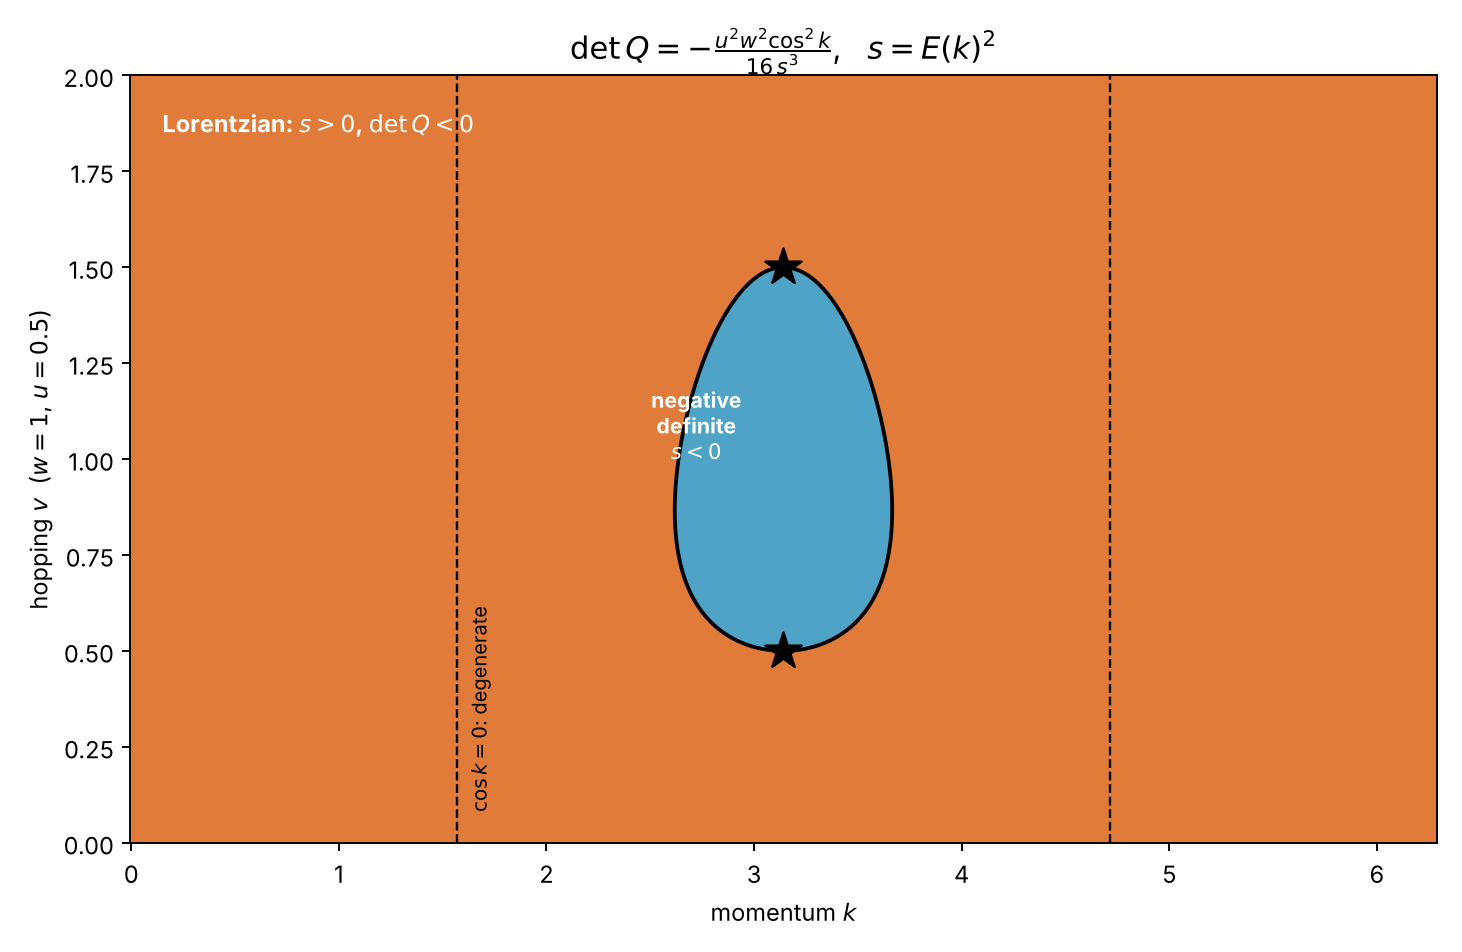
\includegraphics[width=0.84\textwidth]{../figures/fig05_metric_signature.png}
\caption{The opened plane's signature from the exact determinant, $u=0.5$, $w=1$. Orange: $s=E^2>0$, Lorentzian. Blue: $s<0$, negative definite. Dashed: $\cos k=0$, degenerate. Black: $s=0$, the exceptional points, where the formula is singular. Stars: the critical points $k=\pi$, $v=w\mp u$.}
\label{fig:signature}
\end{figure}

\paragraph{Entropy on the opened chain.} At the critical point the Rényi-2 coefficient reads $-1.79\to-1.96$ on the $v<w$ side and $-0.88\to-1.09$ on the $v>w$ side, where the fit has not converged; the biorthogonal entropy is complex there, with $\max|\Ima S_2|=6.3$ at $v<w$ \grade{V} (script \texttt{s03b}). A negative fitted coefficient is a property of the biorthogonal entropy convention (Chang, You, Wen and Ryu), not a negative number of channels: a nonnegative census with $N(\xi)=a\log\xi+O(1)$ cannot have $a<0$ \grade{T}.

\subsection{Where opened matter leaves the disk}
Approaching the critical point at fixed $u$, the census levels leave the disk \emph{before} it, inside the gapped phase, at $v_{\mathrm{exit}}=0.468$ for $u=0.5$ \grade{V}. At every critical point tested ($u=0.2,\dots,0.7$) a level sits at $\Ima W=\pi$ exactly: the half-turn of the unbound nuclei.

\begin{proposition}[the Petermann factor and the exit line]\label{prop:petermann}
For $H=d\cdot\sigma$, $d\in\mathbb C^3$, $E^2=d\cdot d\neq0$, the band projectors $P_\pm=\tfrac12(I\pm H/E)$ are rank-one idempotents with $K_\pm=\Tr P_\pm^*P_\pm=\tfrac12(1+\sum|d_j|^2/|E|^2)\ge1$. On the PT-symmetric chain with $A=v^2+w^2-u^2>|2vw|=|B|$, $K(k)=1+u^2/E(k)^2$ and
\[
\langle K\rangle=1+\frac{u^2}{\sqrt{A^2-B^2}}=1+\frac{u^2}{E(0)E(\pi)},\qquad\langle K\rangle=2\iff E(0)E(\pi)=u^2. \quad\grade{T}\grade{L}
\]
\end{proposition}
\begin{proof}
$H^2=E^2I$ and $\Tr H=0$ give idempotence and unit trace; $\Tr H^*H=2\sum|d_j|^2$; $|E|^2=|\sum d_j^2|\le\sum|d_j|^2$. Here $\sum|d_j|^2=|q|^2+u^2$ and $|E|^2=|q|^2-u^2$. The average uses $\frac1{2\pi}\int_0^{2\pi}\frac{dk}{A+B\cos k}=(A^2-B^2)^{-1/2}$ and $\sqrt{A^2-B^2}=\sqrt{A+B}\sqrt{A-B}=E(0)E(\pi)$ (A.14).
\end{proof}
Checked to $3.6\times10^{-14}$. Predicted from $\langle K\rangle=2$ at three values of $u$ not used before, the exits are $0.7474014$, $0.5291503$, $0.2357262$; measured, $0.7474015$, $0.5291503$, $0.2357262$ (differences $4\times10^{-8}$ and below; block $40$, block-independence from \texttt{s04b}) \grade{V}. The equivalence concerns the band average; that a finite block census crosses the rim at the same parameter is a separate statement, which carries its block, boundary conditions, filter, error and limit.

\paragraph{The limits of the exit law.} Three findings scope it, and they belong in the statement.
\begin{enumerate}
\item On the cone paper's band made one-dimensional, $d=(t_1+\cos k,\sin k,m+i\gamma)$, a mass term moves the exit far earlier ($\langle K\rangle\approx1.01$–$1.06$ at the returned exits); the law holds only at $m=0$, the SSH class \grade{V}.
\item The returned exit depends on the endpoint filter that discards levels with $\nu$ near $0$ or $1$ (ring $2000$, block $40$, $t_1=0.5$, principal logarithm):
\begin{center}\small
\begin{tabular}{rcccc}\toprule
filter $\delta$ & massive $\gamma_{\mathrm{exit}}$ & massive $\langle K\rangle$ & massless $\gamma_{\mathrm{exit}}$ & massless $\langle K\rangle$\\\midrule
$10^{-6}$ & $0.271636929$ & $1.057972846$ & $0.474341649$ & $2.000000002$\\
$10^{-8}$ & $0.271636929$ & $1.057972846$ & $0.474341649$ & $2.000000002$\\
$10^{-9}$ & $0.169169932$ & $1.022352491$ & $0.474341649$ & $2.000000002$\\
$10^{-10}$ & $0.169169932$ & $1.022352491$ & $0.474341467$ & $1.999995744$\\
$10^{-12}$ & $0.122791366$ & $1.011745220$ & $0.474227956$ & $1.997345192$\\\bottomrule
\end{tabular}
\end{center}
The eigenpair residuals are at most $4.4\times10^{-15}$ while the eigenvector condition numbers run $135$ to $575$; a small residual is not an eigenvalue error bound for a nonnormal matrix \grade{V} (scripts \texttt{g\_incoming\_exit\_filter}, \texttt{g\_incoming\_exit\_residuals}, independent band-projector assembly; Figure~\ref{fig:exit}). The massive exit is not yet a filter-independent threshold; the massless exit holds through $10^{-9}$ and shifts below.
\item With $w=0$ and $v^2=2u^2$ the band average is exactly 2, yet no block level ever leaves $\{0,1\}$ \grade{T}: $H(k)$ is then constant, the real-space projector is a direct sum of identical cell projectors, and any union of whole cells compresses to an idempotent. The average alone does not force an exit; the coupling and the partition are part of the law.
\end{enumerate}
What survives: on the coupled PT-symmetric chain with whole-cell blocks and filters through $10^{-9}$, the census leaves the disk where $E(0)E(\pi)=u^2$, to $4\times10^{-8}$ \grade{V}; why it does is open \grade{C}.

\subsection{The offset as the exit's clock}
For opened matter each level's offset $\tau_\nu=\Log((1-\nu)/\nu)$ is complex, and the rotation used above is $|\Ima\tau_\nu|/\pi$. The disk exit is where some level's signed offset has turned a quarter, and the critical point where one has turned a half.

The author's closed form for the endpoint offset of a gapped chain is $2\operatorname{artanh}(v/\sqrt{E_{\min}E_{\max}})$ (\emph{The Offset Belongs to the Boundary}). On the opened chain write $\gamma=u/\sqrt{E(0)E(\pi)}\ge0$, so that $\langle K\rangle-1=\gamma^2$ exactly (to $2.8\times10^{-14}$ over $20\,000$ random parameters). The continuation that carries the opening sends the argument to $i\gamma$:
\begin{equation}
\tau_{\mathrm{end}}=2\operatorname{artanh}(i\gamma)=2i\arctan\gamma,\qquad\Gamma_{\mathrm{end}}=\tanh\frac{\tau_{\mathrm{end}}}2=i\gamma,\qquad\langle K\rangle=1+\gamma^2=\sec^2\Big(\tfrac12\Ima\tau_{\mathrm{end}}\Big).
\label{eq:quarter}
\end{equation}
At $\langle K\rangle=2$, $\gamma=1$: $\tau_{\mathrm{end}}=i\pi/2$ is finite, and $\Gamma_{\mathrm{end}}=i$ lies on the rim \grade{T}\grade{V}. The exit line is a quarter turn of this offset, on the imaginary axis of the disk; the real-argument expression $2\operatorname{artanh}\gamma$, which diverges at $\gamma=1$, belongs to a different chart and is not this continuation (A.15). The quarter-turn is not, however, a description of the census rotation away from the exit. Tested before the run with a kill condition, at $u=0.3,0.5,0.7$ and three points on the approach, the measured rotation sits $4\times10^{-6}$ to $3.4\times10^{-2}$ above $\Ima\tau_{\mathrm{end}}$, independent of block size; the two meet only at the quarter-turn. The level carrying the largest rotation is often one with $\nu$ within $10^{-7}$ of an endpoint, the ill-conditioned levels of the filter table \grade{V} (script \texttt{s11}). Whether a biorthogonal form of $\dot\tau^2\le4gS$ governs the rotation is open \grade{C}.

\begin{figure}[!htbp]\centering
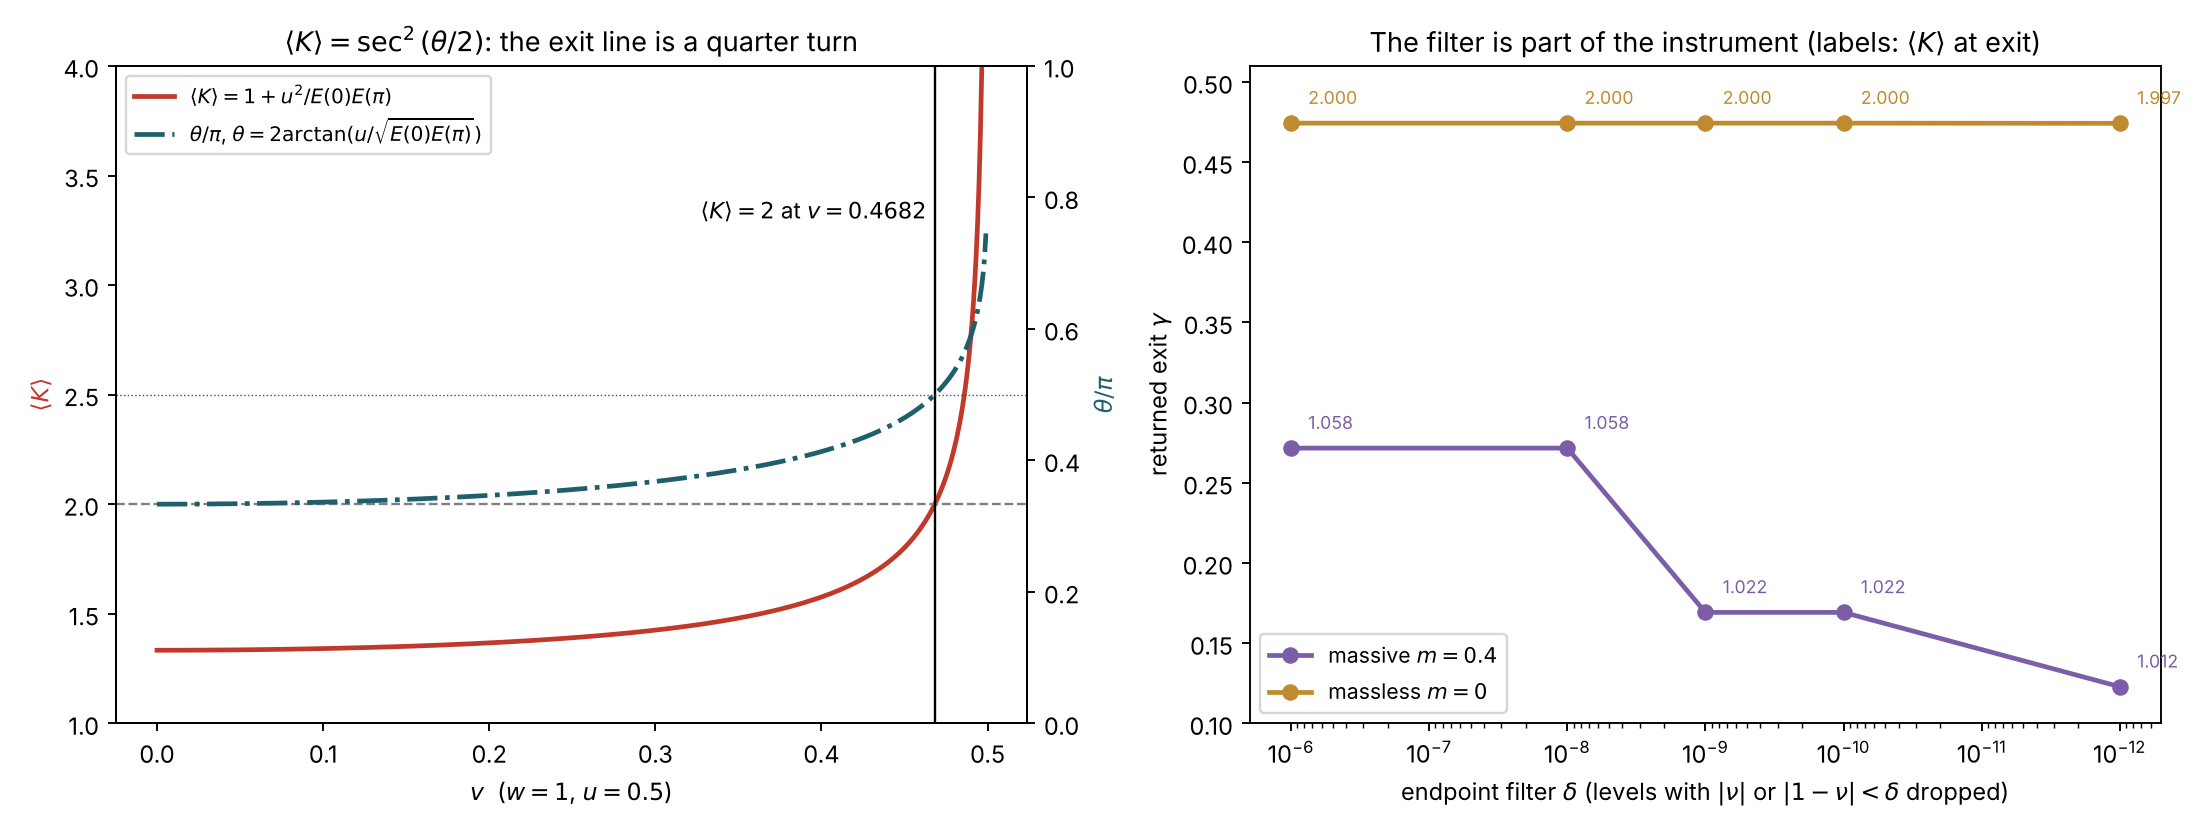
\includegraphics[width=\textwidth]{../figures/fig07_exit_and_filter.png}
\caption{Left: $\langle K\rangle=1+u^2/E(0)E(\pi)$ and the continued endpoint phase $\theta=2\arctan(u/\sqrt{E(0)E(\pi)})$ along $v$ ($u=0.5$, $w=1$); $\langle K\rangle=2$ exactly where $\theta=\pi/2$, at $v=0.4682$, beside the measured census exit $0.468$. Right: the exit returned at five endpoint filters; labels give $\langle K\rangle$ at the returned exit.}
\label{fig:exit}
\end{figure}

\subsection{Two kinds of wall}
The black-hole paper sorts walls by what the spectrum does along a physical path (ed.~10, §8). At a \emph{spectral} wall a real pair turns complex: the unfolding coordinate is real on one side and imaginary on the other, and the Jordan block at the wall is a property of the operator in every frame. At a \emph{geometric} wall the spectrum stays real on both sides, and the Jordan block lives only in a folded chart \grade{S}. Opened matter's exit is spectral: on $\sigma_x+i\gamma\sigma_z$ the eigenvalues $\pm\sqrt{1-\gamma^2}$ turn imaginary at $\gamma=1$, the left–right overlap collapses as $\sqrt{1-\gamma^2}$, and the Petermann factor is $(1-\gamma^2)^{-1}$. At such a point a single eigenprojector grows like $|A_{12}|/\mathrm{gap}$ while the pair projector, its contour trace (count $2$) and the trace-log ledger stay exact (ed.~10 §4; in its two-mode ringdown model the single excitation factors reach $391$ with nearly opposite phases while their sum stays fixed) \grade{V}\grade{S}. The band-averaged Petermann factor of §\ref{sec:opened} is the census-side reading of the same mechanism: what grows is the non-orthogonality of single levels, and what crosses the rim is the record of the pair.

\section{The even and odd halves}\label{sec:parity}
For an involution $J$ ($J^2=\mathrm{id}$) on a space of states or operators, every readout splits as $f=f_{\mathrm{even}}+f_{\mathrm{odd}}$ with $f_{\mathrm{even}}=\tfrac12(f+f\circ J)$ and $f_{\mathrm{odd}}=\tfrac12(f-f\circ J)$. Odd parts vanish at fixed points and under $J$-symmetric pairing or averaging; they do not become false, and they need not vanish merely because a surface is called a wall. Each claim below names its $J$.

\begin{proposition}[complement parity]\label{prop:parity}
(i) Under occupation complement $\nu\mapsto1-\nu$: $\nu(1-\nu)$, every census and every boundary coordinate $\Gamma_b$ are even; $\Gamma=1-2\nu$ and the offset $\tau$ are odd. (ii) For an orthogonal projector $P$ and Hermitian Grassmannian tangents $V,W$ (block off-diagonal), the map $P\mapsto I-P$, $(V,W)\mapsto(-V,-W)$ sends $Q=\Tr(PVW)$ to $\overline Q$: the quantum metric $g=\Rea Q$ is even and the curvature $\Omega=2\Ima Q$ is odd. (iii) Under the adjoint, $R_{H^*}(z)=R_H(\bar z)^*$ for the resolvent $R_H(z)=(z-H)^{-1}$; it is not in general $-R_H(z)$. A Bargmann invariant under complex conjugation has even real part and odd imaginary part. \grade{T}\grade{V}
\end{proposition}
\begin{proof}
(i) is direct. (ii) First, $\overline Q=\Tr((PVW)^*)=\Tr(WVP)=\Tr(PWV)$. Off-diagonality means $(I-P)V=(I-P)VP$ and $PW=PW(I-P)$, so $\Tr((I-P)VW)=\Tr((I-P)VPW)=\Tr(PW(I-P)V)=\Tr(PWV)=\overline Q$. The image of $Q$ is $\Tr((I-P)(-V)(-W))=\Tr((I-P)VW)=\overline Q$; summing the two traces also gives $\Tr(VW)=2\Rea Q$. (iii) $(\bar z-H)^{-1*}=(z-H^*)^{-1}$.
\end{proof}
Script \texttt{s13} checks (ii) on 200 random projectors to $1.5\times10^{-14}$ and confirms that the minus-sign law for the resolvent fails on a random control (largest violation $18.9$). This is where the census and the offset meet as one object: the census is the even half of the boundary log-determinant and the offset its odd half, ``the gauge without its sign'' and ``the clock face'' (atlas W9, B202, B204). Under the same complement, IQGT's metric is the even half and its Berry curvature the odd half of one Hermitian form, which is why the curvature bound $|\Omega(V,W)|\le2\sqrt{g(V,V)g(W,W)-g(V,W)^2}$ follows from the positivity of the even part alone (A.17) \grade{T}. The broader reading, that across the author's programme what survives a wall's involution is the even part and what is lost is the odd part, is a reading of particular cases, each with its own $J$, and is graded so \grade{H}. The black-hole paper's orientation sign, invisible to the Gram observer and kept by the oriented cover, is one such case \grade{S}.

\section{What is proved, what is measured, what is open}\label{sec:status}
\begin{center}\small
\begin{longtable}{p{0.68\textwidth}l}\toprule
Statement & grade\\\midrule\endhead
Zero and span free; a ratio needs a physical zero & \grade{T}\\
Census logarithm with $A=2c/\pi^2$ (given equal spacing and Calabrese–Cardy) & \grade{T}, \grade{V} at $c=1,\tfrac12$\\
$\Gamma=\tanh(\varepsilon/2)=1-2\nu$; $\int H\,d\varepsilon=\pi^2/3$ & \grade{T}\grade{L}\\
Cayley domain with explicit branch; pole only at $z=-1$ & \grade{T}\grade{L}\\
Offset = summed rapidity = log-odds empty/full (quasi-free) & \grade{T}\\
Weight between: defect split, $0\le X\le F\le\tfrac14$, two-sided, census comparison, trace estimate & \grade{T}\grade{L}(core)\\
$\Gamma_b=\sqrt{1-4\lambda}$; $=|1-2\nu|$ on a pure state & \grade{T}\grade{L}\\
Operator-norm stability with certified margin; near-projector comparison; Hölder coordinate & \grade{T}, \grade{V}\\
Same local block, different weight between; three census counterexamples & \grade{T}\\
Number covariance; $4\Tr X_A\le I_G\le\Tr X_A/\delta(1-\delta)$; census bound & \grade{T}, \grade{V}\\
Offset speed limit $\dot\tau^2\le4gS$ & \grade{T}\\
Equal census, offset and coupling; opposite offsets, both saturating & \grade{T}\grade{V}\\
Warm ring: boundary count $2\to0$ with $\Tr X_A=0.170835>0$ & \grade{V}\\
Peel steps add like velocities; Ising census ladder = constant peel step & \grade{T}\grade{L}, \grade{V}\\
Gap step reflects with the peel coordinate & \grade{T}\grade{V}\\
Schur–Cayley boundary: passive inside, matched load at centre & \grade{T}; horizon \grade{S}\\
Hawking fermion record $\tau=\hbar\omega/k_BT_H$, $\Gamma=\tanh(\hbar\omega/2k_BT_H)$ & \grade{T}\grade{V}; reading \grade{H}\\
Anchored coordinate equivalence; helium $\Gamma_0=0.377575$ & \grade{T}\grade{L}, \grade{lit}\\
Scale blindness; last peel step $5/(8Z-5)$, $Z\ge2$ & \grade{T}\grade{L}\\
Unique neutral Saha state; responses; scaling; atomic record insufficiency & \grade{T}\grade{L}(three charges)\\
Gas carries the peel back; partition correction; conditioning & \grade{T}, \grade{R}, \grade{V}\\
Unbound nuclei outside; rim distance $2s/(S_{\mathrm{next}}-s)$; half turn & \grade{T}\grade{L}, \grade{V}\grade{lit}\\
Reduced equation with hidden source; channel measure & \grade{T}\\
Equal spectrum and footprint, different survival; same kernel, different source & \grade{T}\grade{V}\\
Finite moments do not fix response; readout dependence & \grade{T}\grade{L}($m=3$), \grade{V}\\
Kinetic witness: same density, flow, stress; $\Delta n\propto\sin^3$; reset factor & \grade{T}\\
ANG1–ANG3 exact; ANG4 $E^-=k^2\kappa^2/3$ & \grade{T}, \grade{V}\\
Opened idempotent: $Y_A=A-A^2$, radial census survives, positivity does not & \grade{T}\grade{L}\\
$\det Q=-u^2w^2\cos^2k/16s^3$: Lorentzian iff $s>0$, $\cos k\neq0$ & \grade{T}\grade{V}\\
Petermann factor; $\langle K\rangle=1+u^2/E(0)E(\pi)$ & \grade{T}\grade{L}\\
Continued endpoint offset $2i\arctan\gamma$; $\Gamma_{\mathrm{end}}=i$ on the rim at $\langle K\rangle=2$ & \grade{T}\\
Opened matter exits before critical at $E(0)E(\pi)=u^2$ (PT class, whole cells, filters to $10^{-9}$) & \grade{V}\\
Complement parity: census even, offset odd; metric even, curvature odd & \grade{T}\grade{V}\\
What survives a wall is the even half & \grade{H}\\\bottomrule
\end{longtable}
\end{center}
Open: why the census rotation meets the offset quarter-turn only at the exit, which needs conditioned eigenvalues for the near-endpoint levels; a proof that the exit happens at $\langle K\rangle=2$ on the coupled chain; a definition of the massive exit with a controlled limit in filter, ring and block size and the order of limits stated, using conditioning and error bounds rather than an assumed error expansion; a biorthogonal speed limit for the complex offset; convergence on the $v>w$ side; the infinite-dimensional limit of the chain's Henrici departure; placing nuclear resonances with their widths on the chart; a second non-unitary model of a different kind; an empirical gas inverse on a real specimen with measured populations, $n_e$ and partitions; a typed map from the speed limit to the record of a physical system beyond the projector constructions here.

\section*{Sources}
\small\sloppy
J.~Beasley, \emph{Matter at a Scale: Zero, Span, and the Logarithm Between Them}, v5 (2026), doi:10.5281/zenodo.22019893.
J.~Beasley, \emph{VOTKP: The Vector of Traits Kept under Peeling}, v2.9 (2026), doi:10.5281/zenodo.23340757.
J.~Beasley, \emph{The Offset Belongs to the Boundary}, v31 (2026), doi:10.5281/zenodo.22555919.
J.~Beasley, \emph{The Offset Speed Limit}, v1.1 (2026).
J.~Beasley, \emph{The Weight Between}, v2.3 (2026).
J.~Beasley, \emph{The Angle Between the Rails} (2026).
J.~Beasley, \emph{A Measured Lorentzian Cone in Non-Hermitian Quantum Geometry}, v8 (2026).
J.~Beasley, \emph{Beyond the Event Horizon: What Survives at a Rigidity Wall}, edition 10 (2026).
J.~Beasley, \emph{Intrinsic Quantum Geometric Tensor on the Grassmannian and Spectral Lower Bounds on Dissipation}, doi:10.5281/zenodo.20768258.
J.~Beasley, \emph{Light Keeps the Ledger}, research edition 7.2 (2026).
J.~Beasley, \emph{Matter, Gases and VOTKP: Formal Research Edition}, 3 November 2026 (prepared with OpenAI tools), repository \texttt{matter-disk/external/gpt\_formal\_20261103}.
J.~Beasley, Physics Atlas v7 (B1–B207) and Atlas II (W1–W9).
P.~Calabrese and J.~Cardy, Entanglement entropy and quantum field theory, J.\ Stat.\ Mech.\ (2004) P06002.
I.~Peschel, Calculation of reduced density matrices from correlation functions, J.\ Phys.\ A 36 (2003) L205.
I.~Peschel and V.~Eisler, Reduced density matrices and entanglement entropy in free lattice models, J.\ Phys.\ A 42 (2009) 504003.
M.~M.~Wolf, F.~Verstraete, M.~B.~Hastings and J.~I.~Cirac, Area laws in quantum systems: mutual information and correlations, Phys.\ Rev.\ Lett.\ 100 (2008) 070502.
P.-Y.~Chang, J.-S.~You, X.~Wen and S.~Ryu, Entanglement spectrum and entropy in topological non-Hermitian systems and nonunitary conformal field theory, Phys.\ Rev.\ Research 2 (2020) 033069.
A.~Unsöld, Ann.\ Phys.\ 387 (1927) 355 (the $\tfrac58Z$ repulsion integral).
K.~S.~Thorne, R.~H.~Price and D.~A.~Macdonald (eds.), \emph{Black Holes: The Membrane Paradigm}, Yale (1986).
F.~G.~Kondev et al., The NUBASE2020 evaluation of nuclear physics properties, Chin.\ Phys.\ C 45 (2021) 030001.
A.~Kramida et al., NIST Atomic Spectra Database (ionization energies), accessed through the VOTKP v2.9 package.
\normalsize
